\documentclass[12pt]{report}
\usepackage[a4paper]{geometry}
\usepackage[myheadings]{fullpage}
\usepackage{fancyhdr}
\usepackage{lastpage}
\usepackage{graphicx, wrapfig, subcaption, setspace, booktabs}
\usepackage[T1]{fontenc}
\usepackage[font=small, labelfont=bf]{caption}
\usepackage{fourier}
\usepackage[protrusion=true, expansion=true]{microtype}
\usepackage[english]{babel}
\usepackage{sectsty}
\usepackage{url, lipsum}
\usepackage{listings}
\usepackage{float}
\usepackage{todonotes}
\usepackage{stmaryrd}
\usepackage{amsfonts}
\usepackage{amsmath}
\graphicspath{{images/}}

\lstset{
	basicstyle=\ttfamily,
	columns=fullflexible,
	frame=single,
	breaklines=true,
	postbreak=\mbox{\textcolor{red}{$\hookrightarrow$}\space},
}

\usepackage{hyperref}
\hypersetup{
	colorlinks,
	citecolor=black,
	filecolor=black,
	linkcolor=black,
	urlcolor=black
}

\newcommand{\HRule}[1]{\rule{\linewidth}{#1}}
\onehalfspacing
\setcounter{tocdepth}{5}
\setcounter{secnumdepth}{5}

%-------------------------------------------------------------------------------
% HEADER & FOOTER
%-------------------------------------------------------------------------------
\pagestyle{fancy}
\fancyhf{}
\setlength\headheight{15pt}
\fancyfoot[R]{Page \thepage\ of \pageref{LastPage}}
%-------------------------------------------------------------------------------
% TITLE PAGE
%-------------------------------------------------------------------------------

\begin{document}
	
	\title{ \normalsize \textsc{Large-Scale Data Analysis Techniques}
		\\ [2.0cm]
		\HRule{0.5pt} \\
		\LARGE \textbf{\uppercase{A Review on Multi-Label Learning Algorithms}}
		\HRule{2pt} \\ [0.5cm]
		\normalsize \today \vspace*{5\baselineskip}}
	
	\date{}
	\author{
		Nikiforos Pittaras, M1422\\
		Chrysoula Themeli, M1423 \\ 
		National and Kapodistrian University of Athens\\
		Department of Informatics and Telecommunications }
	
	\maketitle
	\tableofcontents
	\listoffigures
	\newpage
	
	%-------------------------------------------------------------------------------
	% Section title formatting
	\sectionfont{\scshape}
	%-------------------------------------------------------------------------------
	
	%-------------------------------------------------------------------------------
	% Summary of the paper
	%-------------------------------------------------------------------------------
	
	\section*{Introduction}
	\addcontentsline{toc}{section}{Introduction}
	
	\subsection*{Multi-label learning}
	\addcontentsline{toc}{subsection}{Multi-label learning}
	The paper "A Review on Multi-Label Learning Algorithms" analyzes the
  multi-label learning field in supervised classification. Supervised
  classification trains a model $f: X \rightarrow Y$ and for each pair
  $f(x_i,y_i)$, it outputs a real number $r$ that represents the confidence that
  label $y_i$ characterizes $x_i$. Given $r$ and a thresholding scheme, labels
  are marked as relevant or not relevant to the input data vector $x_i$ (e.g.
  for $r$ representing probability estimates, $r \in [0,1]$, a simple
  thresholding function is $t(x_i) = 0.5$. In other words, labels with outputs
  greater than $0.5$ are assigned to $x_i$ by our model). Standard, single-label learning maps an
  example to a single label, completely ignoring multiple semantics that
  real-objects usually have. On the other hand, multi-label learning allows an
  example/instance $x_i$ to be mapped to more than one label, i.e. to any label
  vector which is a subset of $Y$. However, this results to an exponentially growing search space, since
  the latter depends on the size of the powerset of $Y$, 
  $|\mathbb{P(Y)}| = 2^{|Y|}$.
	
	One straightforward solution is to exploit label correlations. Real objects
  are usually characterized by similar concepts. For example, if an article is
  characterized by label "football" it follows that it will be also
  characterized by the term "sports" and it is likely that it will be labeled
  with ``crowd'' or ``entertainment''. On the other hand, the label "science"
  will be likely to be irrelevant. In order to exploit such kind of label
  correlations, three different algorithm strategies are examined:
	
	\begin{itemize}
		\item \textbf{First-order strategies: }These algorithms ignore label
      correlations and perform a "one-vs-all" strategy. They often transform a
      multi-label problem into multiple single-label problems, combining the
      result in an aggregation-like manner. Algorithms of this category are
      simple, scalable, have the capability of parallel implementation, but
      offer suboptimal performance.
		\item \textbf{Second-order strategies: }Algorithms in this category consider
      \emph{pairwise} label correlations, i.e. tuples of labels. Having a good
      trade-off between generalization performance and scalability, they
      generally outperform first-order strategies but their limited exploration
      of the label dependency space leads to lacking performance in some real
      world applications.
		\item \textbf{High-order strategies: }These algorithms capture a high degree
      of label correlations, having a large comlexity and strong modeling
      capabilities. This of course leads to increased performance but renders them computationally demanding and less scalable.
	\end{itemize}
	
	\subsection*{Evaluation metrics}
	\addcontentsline{toc}{subsection}{Evaluation metrics}

	With respect to performance evaluation, traditional single-label evaluation metrics are extended to
  incorporate the multi-labeled output. This extension is categorizable into two
  groups. One with respect to the expansion ``axis'' (across examples or labels)
  and the task type (classification or ranking).

    Before proceeding with the metrics, true positive(TP), false positive(FP),
    true negative (TN) and false negative (FN) of label $y_j$ will be defined:
		\begin{itemize}
			\item \emph{True positive: } $TP_j = |\{x_i | y_j \in Y_i \wedge y_j \in h(x_i), 1 \leq i \leq p \}|$
			\item \emph{False positive: }$FP_j = |\{x_i | y_j \notin Y_i \wedge y_j \in h(x_i), 1 \leq i \leq p \}|$
			\item \emph{True negative: }$TN_J = |\{x_i | y_j \notin Y_i \wedge y_j \notin h(x_i), 1 \leq i \leq p \}|$
			\item \emph{False negative: }$FN_J = |\{x_i | y_j \in Y_i \wedge y_j \notin h(x_i), 1 \leq i \leq p \}|$
		\end{itemize}

	\begin{itemize}
		\item \textbf{Example-based: }This kind of metrics evaluate multi-labeled performance on each example and then the result is spread to the whole dataset. The metrics are divided into two perspectives:
      \todo{Form them up into a table}
		\begin{itemize}
			\item Classification:
        \begin{table}
          \centering
          \begin{tabular}{cc} 
          \toprule
            one & two \\
          \midrule
            one & two \\
            one & two \\
          \bottomrule
          \end{tabular}
          \caption{Evaluation metrics for multi-label learning}
          \label{label:evaluation_metrics}
        \end{table}

			\begin{itemize}
				\item Precision: $P(h) = \frac{1}{p} \sum_{i=1}^{p} \frac{|Y_i \cap h(x_i)|}{h(x_i)|}$
				\item Recall: $R(h) = \frac{1}{p} \sum_{i=1}^{p} \frac{|Y_i \cap h(x_i)|}{|Y_i}$
        \item Subset Accuracy:  $SA(h) = \frac{1}{p} \sum_{i=1}^p \llbracket h(x_i) = Y_i \rrbracket$
				\item Hamming Loss: $H(h) = \frac{1}{p} \sum_{i=1}^{p} [h(x_i)\Delta Y_i] $
				\item Accuracy: $A(h) = \frac{1}{p} \sum_{i=1}^{p} \frac{|Y_i \cap h(x_i)|}{|Y_i \cup h(x_i)|}$
				\item $F^ \beta$ -metric:  $F^ \beta _{exam} (h) = \frac{(1+ \beta ^2) \cdot Precision_{exam}(h) \cdot Recall_{exam}(h)}{\beta ^2 \cdot Precision_{exam}(h) + Recall_{exam}(h)}$
			\end{itemize}
			\item Ranking:
			\begin{itemize}
				\item One-error: $one-error(f) = \frac{1}{p} \llbracket [argmax_{y \in Y}f(x_i,y)] \notin Y_i \rrbracket$
				\item Coverage:  $coverage(f) = \frac{1}{p} \sum_{i=1}^{p} max_{y \in Y_i} rank_f(x_i,y) - 1$
				\item Ranking loss: $rloss(f) = \frac{1}{p} \sum_{i=1}^{p} \frac{1}{|Y_i| {\overset{\sim}{|Y_i|}}} |\{(y', y'') | f(x_i,y') \leq f(x_i,y''), (y', y'') \in Y_i \times {\overset{\sim}{|Y_i|}} \}| $ 
				\item Average Precision:  $agvprec(f) = \frac{1}{p} \sum_{i=1}^{p} \frac{1}{|Y_i|} \sum_{y \in Y_i} \frac{|\{y' | rank_f(x_i,y') \leq rank_f(x_i,y), y' \in Y_i\}|}{rank_f(x_i,y)}$
			\end{itemize}
		\end{itemize}
  \item \textbf{Label-based: }
		The label-based metrics are also separated in two perspectives:
		\begin{itemize}
			\item Classification: Let $B(TP_j, FP_j, TN_J, FN_J)$ represent some specific binary classification metric $(B \in \{Accuracy, Precision, Recall, F^ \beta \})$. The metrics from classification perspective are the following:
			\begin{itemize}
				\item Macro-averaging: $B_{macro}(h) = \frac{1}{q} \sum_{1}^{q} B(TP_j, FP_j, TN_J, FN_J)$
				\item Micro-averaging: $B_{micro}(h) = B(\sum_{1}^{q}TP_j, \sum_{1}^{q}FP_j, \sum_{1}^{q}TN_j, \sum_{1}^{q}FN_j)$
			\end{itemize}
			\item Ranking:
			\begin{itemize}
				\item \emph{AUC macro: }$AUC_{macro} = \frac{1}{q} \sum_{1}^{q} \frac{|\{(x', x'') | f(x',Y_j) \geq f(x'',Y_j), (x',x'') \in Z_j \times \overset{\sim}{|Z_j|} \}|}{|Z_j|{\overset{\sim}{|Z_j|}}}$
				\item \emph{AUC micro: }$AUC_{micro} = \frac{|\{(x',x'',y',y'') | f(x',y') \geq f(x'',y''), (x',y') \in S^+, (x'',y'') \in S^- \}|}{|S^+||S^-|}$
			\end{itemize}
		\end{itemize} 
	\end{itemize}
	
	\section*{Multi-label learning algorithms}
	\addcontentsline{toc}{section}{Multi-label learning algorithms}
	In this paper, eight representative multi-label algorithms are presented and analyzed, seleceted with respect to below criteria:
	\begin{itemize}
		\item[$\checkmark$] Broad, noteworthy and/or unique characteristics
		\item[$\checkmark$] Primitive impact (i.e. leads to a number follow-up related methods)
		\item[$\checkmark$] Favorable influence (popular and/or highly-cited) 
	\end{itemize}
	
	The algorithms to be presented are grouped in two categories:
	\begin{itemize}
		\item \textbf{Problem Transformation Methods: }Algorithms of this category
      transform the multi-labeled problem into into other well-established
      single-labeled learning scenarios, fusing the results into a multi-label output (``Fit data to algorithm'' philosophy)
		\item \textbf{Algorithm Adaptation Methods: }Here, algorithms adapt popular learning techniques to deal with multi-label data directly ("Fit algorithm to data" philosophy)
	\end{itemize}

	\subsection*{Problem Transformation Methods}
	\addcontentsline{toc}{subsection}{Problem Transformation Methods}
	\begin{figure}[H]
		\centering
		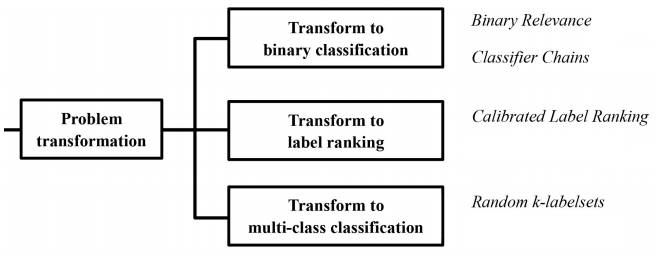
\includegraphics[width=0.9\textwidth]{pt.png}
		\caption{Problem Transformation Algorithms}
		\centering
	\end{figure}

	\subsubsection*{Binary Relevance}
	\addcontentsline{toc}{subsubsection}{Binary Relevance}
	Binary relevance (BR) decomposes the multi-learning problem into $q$
  independent binary classification problems, each of them corresponding to a
  possible label in the label-set $Y$. The first task is to construct a
  corresponding binary training set for each label, on which a binary learning
  algorithm is used in order to train the binary classifier that discriminates
  class $y_j$, i.e. $h_j(\cdot)$. Each training instance is involved in the
  learning process of all $q$ classifiers(cross-training strategy), which is
  regarded as positive instance in case of relevant labels and negative
  otherwise. For new instances, the algorithm predicts the relevant labelset by
  querying each binary classifier and combining the relevant labels. A label is
  considered relevant according to the thresholding scheme adopted in the classifier.
	
	This is a first-order approach algorithm, since it ignores completely any
  label associations. However, since an one-vs-rest scheme is used and
  classifiers are built for each label separately, the algorithm has the
  capability of parallel implementation. Finally, this separation renders the
  algorithm sensitive to class-imbalance in the dataset\footnote{The case where
    the number of positives and negatives for a class differs significantly}.
	
	\subsubsection*{Classifier Chains}
	\addcontentsline{toc}{subsubsection}{Classifier Chains}
	The logic of this algorithm is to transform the multi-label learning problem
  into a chain of binary classification problems, using subsequent binary
  classifiers in a chain, built upon the predictions of preceding ones and
  ordered by a permutation function $f_p$. First of all, a binary training set
  is constructed by enriching each instance with the confidence of preceding
  classifiers, which are concatenated with the data vector $x_i$. Moreover, a binary algorithm is used in step $i$ to
  determine whether label $y_i$ label is relevant or not for an instance. For
  unknown instances the algorithm predicts the relevant labels by iteratively
  traversing the classifier chain producing thresholded confidence scores ($\lambda _{\tau(j)}^x \in {-1, +1}$ in the
  same order as within the training process by $f_p$ represents the predicted binary assignment of $y_{\tau(j)}$)
	
	This is a high-order method, that exploits label correlations to a degree, but in a random manner. However, it is highly sensitive to the permutation function, since the classifiers' ordering directly affects the result. One other disadvantage is that iterative operation prevents parallel implementation. Finally, one possible improvement to overcome the affect of classifiers' ordering is to use ensemble schemes.
	
	\subsubsection*{Claibrated Label Ranking}
	\addcontentsline{toc}{subsubsection}{Claibrated Label Ranking}
	This algorithm transforms the learning problem into a label pairwise comparison ranking problem. For $q$ labels, $q(q-1)/2$ binary classfiers are generated by pairwise comparison and a binary algorithm $h_{jk}(x)$ is used. Firstly, training sets $D_{jk}$ are constructing, where $D_{jk}: \{x_i, Y_i | y_j \in Y_i \oplus y_k \in Y_i\}$. The learning system votes for each example and if $h_{jk}(x)>0$, then $x_i$ is associated with label $y_j$, otherwise $y_j$ is irrelevant and $x_i$ is assigned to $y_k$. For unknown instances, classifiers' votes are aggregated and ranked. In addition, a virtual label $y_v$ is used as an artificial splitting point between relevant and irrelevant labels.
	
	This is a second-order approach algorithm using a one-vs-one scheme. The advantage of this method is that it smooths out the class-imbalance problem (where the number of a class positives is much less than the other's class positives). The disadvantage is the number of classifiers is quadratic to $|Y|$, compared to linear for Binary Relevance algorithm. One improvement to this issue is to use pruning methods to reduce the search space.
	
	\subsubsection*{Random k-Labelsets}
	\addcontentsline{toc}{subsubsection}{Random k-Labelsets}
	Random k-labelsets algorithm transforms the multi-label learning problem into an ensemble of multi-class classification problems where each component targets a random subset of $Y$, that appears in $X$ classified with Label Powerset (LP) techniques. In more detail, the multi-label dataset is transformed into single-label data by treating each distinct labelset as a new class. Each training example is reassigned with the new mapped class and classified through regular single-label classification. An instance $x_i$ is assigned to label $y_i$ when the votes received for $y_i$ from the ensemble exceed half the max possible that this label can get. For unseen instances $x$, LP predicts its associated label set $Y$ by querying the prediction of multi-class classifier and then mapping it back to the power set of $Y$.
	
	This is a high-order approach algorithm, utilizing label correlations. However, there are two limitations in terms of practical feasibility: 
	
	\begin{itemize}
		\item[$\diamond$] \emph{Incompleteness: }The algorithm is data-sensitive and cannot generalize to labelsets that do not appear into the training set
		\item[$\diamond$] \emph{Inefficiency: }Large $Y$ implies high training complexity and extremely few training examples for some newly mapped classes.
	\end{itemize}

	To overcome above issues while keeping LP's simplicity, Random k-Labelsets chooses to combine ensemble learning with LP. The latter is invoked only on random k-labelsets (each leading to a multi-class classifier $g_{y^k(l_r)}^+$) to guarantee computational efficiency and then ensemble a number of LP classifiers to achieve predictive completeness. For new instances $x$, two quantities are calculated: $\tau(\textbf{x},y_j)$, which counts the maximum number of votes that $y_j$ can receive from the ensemble and $\mu(\textbf{x},y_j)$, which counts the actual number of votes that $y_j$ receives from the ensemble. Therefore, the predicted labelset is calculated as follows: $Y = \{y_j|\mu(\textbf{x},y_j)/\tau(\textbf{x},y_j)>0.5,  1 \leq j \leq q\}$. This means that when the actual number of votes exceeds half of the maximum number of votes, $y_j$ is considered as a relevant label.For an ensemble created by n k-labelsets, the maximum number of votes on each label is $nk/q$ on average (usually: k=3 and n = 2q). Finally, another way to improve LP is to prune distinct label set in D appearing less than a pre-specified counting threshold.
	
	\subsection*{Algorithm Adaptation Methods}
	\addcontentsline{toc}{subsection}{Algorithm Adaptation Methods}
	
	\begin{figure}[H]
		\centering
		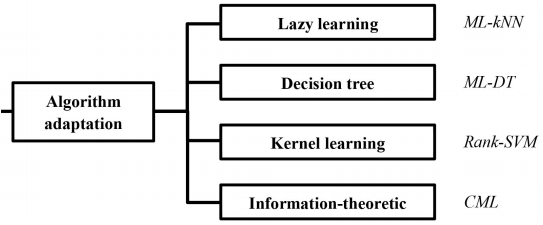
\includegraphics[width=0.9\textwidth]{aa.png}
		\caption{Algorithm Adaptation Methods}
		\centering
	\end{figure}

	\subsubsection*{Multi-Label k-Nearest Neighbor (ML-kNN)}
	\addcontentsline{toc}{subsubsection}{Multi-Label k-Nearest Neighbor (ML-kNN)}
	ML-kNN algorithm adapts k-nearest neighbor techniques utilizing maximum a posteriori (MAP) rule to make prediction by reasoning with the labeling information embodied in the neighbors. For new instances $x$, $N(x)$ represents the set of its k nearest neighbors identified in the dataset (similarity among instances is calculated by Euclidean distance). Let $H_j \equiv (y_j \in Y_i)$, $C_j = \sum_{x_k \in N(x_i)} [\delta(y_j \in Y_k)]$. $C_j$ records the number of x’s neighbors with label $y_j$, while $H_j$ is the event that $\textbf{x}$ has the label $y_j$. Moreover, $P(H_j|C_j)$ is the posterior probability that $H_j$ can be applied in the condition that $\textbf{x}$ has exactly $C_j$ neighbors. Similarly, $P(\neg H_j|C_j)$ needs to be calculated in order to decide if to include $y_j$ in the prediction. This will be computed using the Bayes' theorem:
	
	\begin{center}
		$\frac{P(H_j|C_J)}{P(\neg H_j|C_j)} = \frac{P(H_j) \cdot P(C_j|H_j)}{P(\neg H_j) \cdot P(C_j| \neg H_j)}$
	\end{center}

	Prior probabilities ($P(H_j)$ and $P(\neg H_j)$) are computed via the frequency counting strategy, where a smoothing parameter $s$ is used to control the effect of uniform prior on the estimation (usually $s=1$). In addition, likelyhoods $P(C_j|H_j)$ and $P(C_j| \neg H_j)$ are computed using two frequency arrays:
	\begin{itemize}
		\item $\kappa(r)$, the number of examples labelled $y_j$ with $r$ neighbours labelled $y_j$
		\item $\overset{\sim}{\kappa}(r)$, the number of examples not labelled $y_j$ with $r$ neighbours labelled $y_j$
	\end{itemize}
	 
	This algorithm is a first-order approach using Bayesian reasoning. The decision boundary can be modified on-line when new instances appear. Moreover, Through prior probabilities calculation class-imbalance issue can be overcome. However, since label correlations are ignored, some extensions are proposed that take into account label associations.
	
	\subsubsection*{Multi-Label Decision Tree (ML-DT)}
	\addcontentsline{toc}{subsubsection}{Multi-Label Decision Tree (ML-DT)}
	ML-DT adapts decision tree techniques using multi-label entropy to build a decision tree recursively. Let $T = \{(x_i, Y_i) | 1 \leq i \leq n \}$ be the multi-label dataset with n examples. The algorithm splits the $x$ vector at the feature $l$ that maximizes the information gain criterion. Moreover, dataset $T$ is split on the $l$-th feature valued $\theta$ into branches ($T^-$ \& $T^+$), where $x_{il} \leq \theta, x_i \in T^-$ and $x_{il} > \theta, x_i \in T^+$. This process is invoked recursively by treating each time one of the two branches as the new root node and terminates until some stopping criterion $C$ is met (e.g. child size). Each subset is treated as a new class and single-label entropy is computed. Any new instances are assigned the label of the majority of members of the leaf that they arrive.
	
	In order to ensure low computational cost and high efficiency, the algorithm assumes independence among the labels (first-order approach). However, extended strategies are proposes, such as pruning and ensemble strategies, so as to exploit label correlations as well.
	
	\subsubsection*{Ranking Support Vector Machine (Rank-SVM)}
	\addcontentsline{toc}{subsubsection}{Ranking Support Vector Machine (Rank-SVM)}
	Rank-SVM adapts maximum margin strategy, where $q$ linear classifiers are optimized to minimize empirical ranking loss and enabled to handle nonlinear cases with kernel tricks. The learning system is composed by those classifiers $W = \{w_j,b_j | 1 \leq j \leq q\}$, where $w_j \in \mathbb{R}^d$ and $b_j \in \mathbb{R}$ are the weight vector and the bias
	for the j-th class label $y_j$ respectively. Rank-SVM defines the system’s margin on $(x_i,Y_i)$ by considering its ranking ability on the relevant and irrelevant label pairs of $x_i$ $(y_j,y_k) \in Y_i \times \bar Y_i$, which are separated by a function of their classifiers $h_j, h_k$: $\left<w_j-w_k, x_i \right> + b_j - b_k=0$. When the learning system is capable of properly ranking every relevant-irrelevant label pair for each training example, the classifier will return positive margin. For each new instances $x$, the algorithms retrieves a ranked list of label pairs.
	
	Moreover, non-linear problems can be solved through feature mapping and kernel trick, while convex quadratic programming problems can be solved by any QP solver. This algorithm is a second-order approach using pairwise label associations. Improvements can be achieved by: replacing ranking with hamming loss which can be cast as a general form of	structured output classification, accomplishing thresholding strategy with techniques other than stacking-style procedure and avoiding the problem of kernel selection by employing multiple kernel learning techniques to learn from multi-label data.
	
	 \subsubsection*{Collective Multi-Label Classifier}
	 \addcontentsline{toc}{subsubsection}{Collective Multi-Label Classifier}
	 This algorithm adapts maximum entropy principle, where correlations among labels are encoded as binary random vectors into a joint probability distribution function(pdf) and label correlations are encoded into the joint pdf as constraints. This is a second-order approach, where all label pairs are considered and not just the relevant-irrelevant ones. Let $H_p(x, y)$ represent the information entropy of $(x,y)$ given their distribution $p(\cdot , \cdot)$. The principle of maximum entropy assumes that the distribution best modeling the current state of knowledge is the one maximizing $H_p(x, y)$ subject to a collection K of given facts: $\mathbb{E_p}[f_k(x,y)] = F_k$, where $F_k$ are estimated from the training set. The fact is expressed as constraint on the expectation of  some  function  over. Along with the normalization constraint on $p(\cdot , \cdot)$ , the constrained optimization problem can be solved with standard Lagrange Multiplier techniques. Any unseen instance $x$ is labeled with $Y = \underset{y}{\text{argmax }} P(y | x)$. Exact inference with arg max is only tractable for small label space, otherwise pruning strategies should be applied.
	 
	 \subsection*{Summary of Multi-Label Learning Algorithms}
	 \addcontentsline{toc}{subsection}{Summary of Multi-Label Learning Algorithms}
	 
	 \begin{figure}[H]
	 	\centering
	 	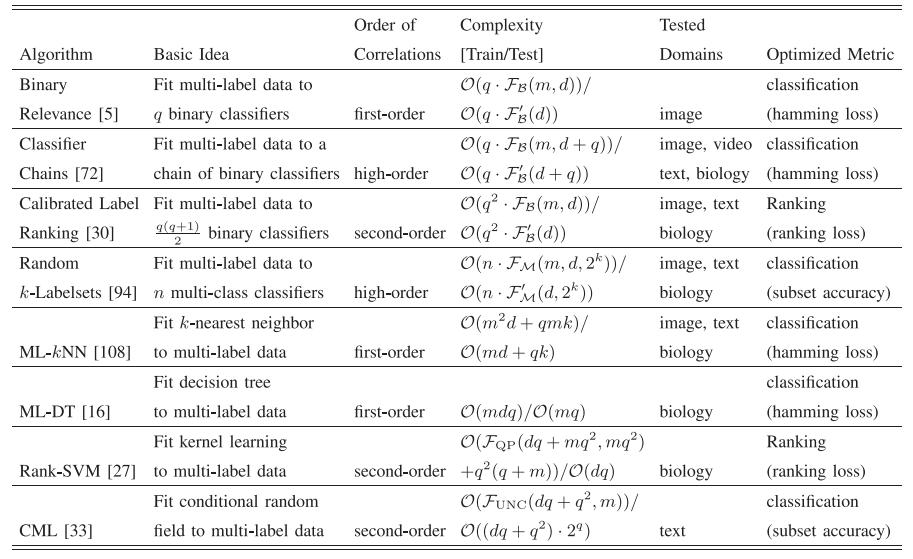
\includegraphics[width=1\textwidth]{summary.png}
	 	\caption{Summary of Multi-Label Learning Algorithms}
	 	\centering
	 \end{figure}
 
 	\section*{Related Learning Methods}
 	\addcontentsline{toc}{section}{Related Learning Methods}
 	Four learning methods are mentioned in this paper, which can be found below:
 	\begin{enumerate}
 		\item \textbf{Multi-instance learning: }This method studies the problem where each example is described by a bag of instances while associated with a single/binary label. Bag is assigned positive label in case of at least one positive member. Finally, it models complex semantics of $x_i$ in input space rather than its output.
 		\item \textbf{Ordinal classification: }This method assumes that labels are related through a natural ordering and instead of explicit class relevance, it assumes an ordering of relevant between labels via a membership vector. Finally, the multi-label problem is transformed into a set of ordinal set of problems.
 		\item \textbf{Multi-task learning: }This method studies the problem where multiple tasks are trained in parallel, sharing information, where knowledge from related tasks is used as an inductive bias to help improve the generalization performance of other tasks. The  tasks can be in the same feature space or different feature spaces, while in multi-label learning all the examples share the same feature space. Finally, in multi-task learning it is not reasonable to have a large number of tasks, while in multi-label learning it is usual to deal with large label space.
 		\item \textbf{Data streams classification: }This method studies the problem	where real-world objects are generated online and processed in a real-time manner. Key factor is to deal with the concept drift problem. Some existing strategies are: classifiers update significantly whenever a new batch of examples arrive, assumption that the influence of past data gradually declines as time evolves or change detector alerting whenever a concept drift is detected.
 	\end{enumerate}
 	
	\section*{Conclusion}
	\addcontentsline{toc}{section}{Conclusion}
	Summarizing all the above, this paper defines the multi-label learning problem, presents 8 multi-label learning representative algorithms and mentiones some additional related learning methods. Some important future goals are the formal characterization on the underlying concept/mechanism on the appropriate usage of label correlations (especially on large output spaces) and also a thorough experimental comparative study to discover the advantages and disadvantages of different multi-label learning algorithms. Below, some online resources on multi-label learning are presented:
	
	\begin{figure}[H]
		\centering
		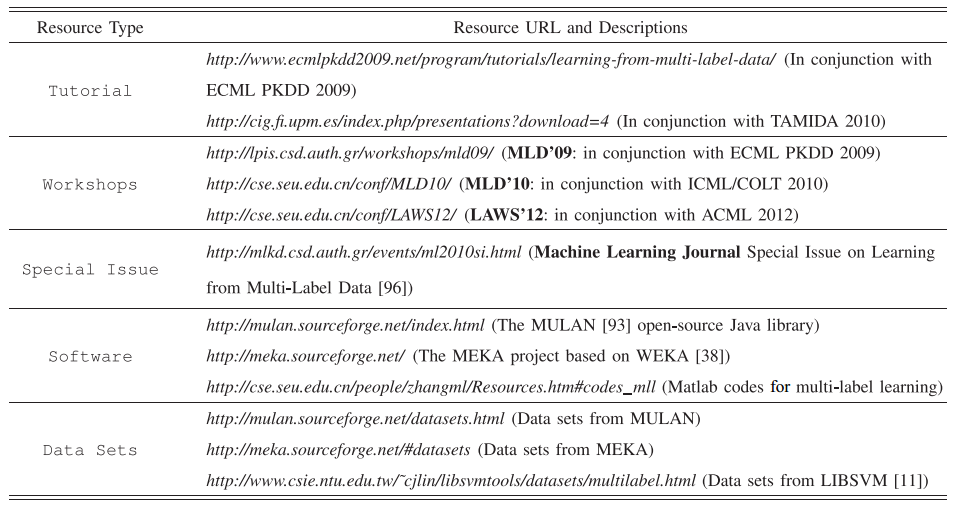
\includegraphics[width=1\textwidth]{online.png}
		\caption{Online resources for Multi-Label Learning}
		\centering
	\end{figure}
	
	%-------------------------------------------------------------------------------
	% REFERENCES
	%-------------------------------------------------------------------------------
	\addcontentsline{toc}{section}{Related Work}
	\renewcommand\bibname{Related Work}
	\begin{thebibliography}{9}
		\bibitem{comp} 
		Madjarov, Gjorgji, et al. "An extensive experimental comparison of methods for multi-label learning." Pattern Recognition 45.9 (2012): 3084-3104
		\bibitem{overview} Tsoumakas, Grigorios, and Ioannis Katakis. "Multi-label classification: An overview." International Journal of Data Warehousing and Mining 3.3 (2006)
		\bibitem{correlations} Zhang, Min-Ling, and Kun Zhang. "Multi-label learning by exploiting label dependency." Proceedings of the 16th ACM SIGKDD international conference on Knowledge discovery and data mining. ACM, 2010
	\end{thebibliography}
\end{document}
